\section{ATLAS Coordinate System} \label{sec:atlas:coordinates}

Using the nominal interaction point as the origin, ATLAS uses a right-handed
coordinate system where the positive $x$-axis points towards the center of the
LHC ring, the positive $y$-axis points upwards, and the positive $z$-axis is
defined by the counter clockwise circulating beam direction as viewed from
above shown in \cref{fig:atlas_geometry} \cite{PERF-2007-01}.  
 
\begin{figure}[!htbp]
  \begin{center}
    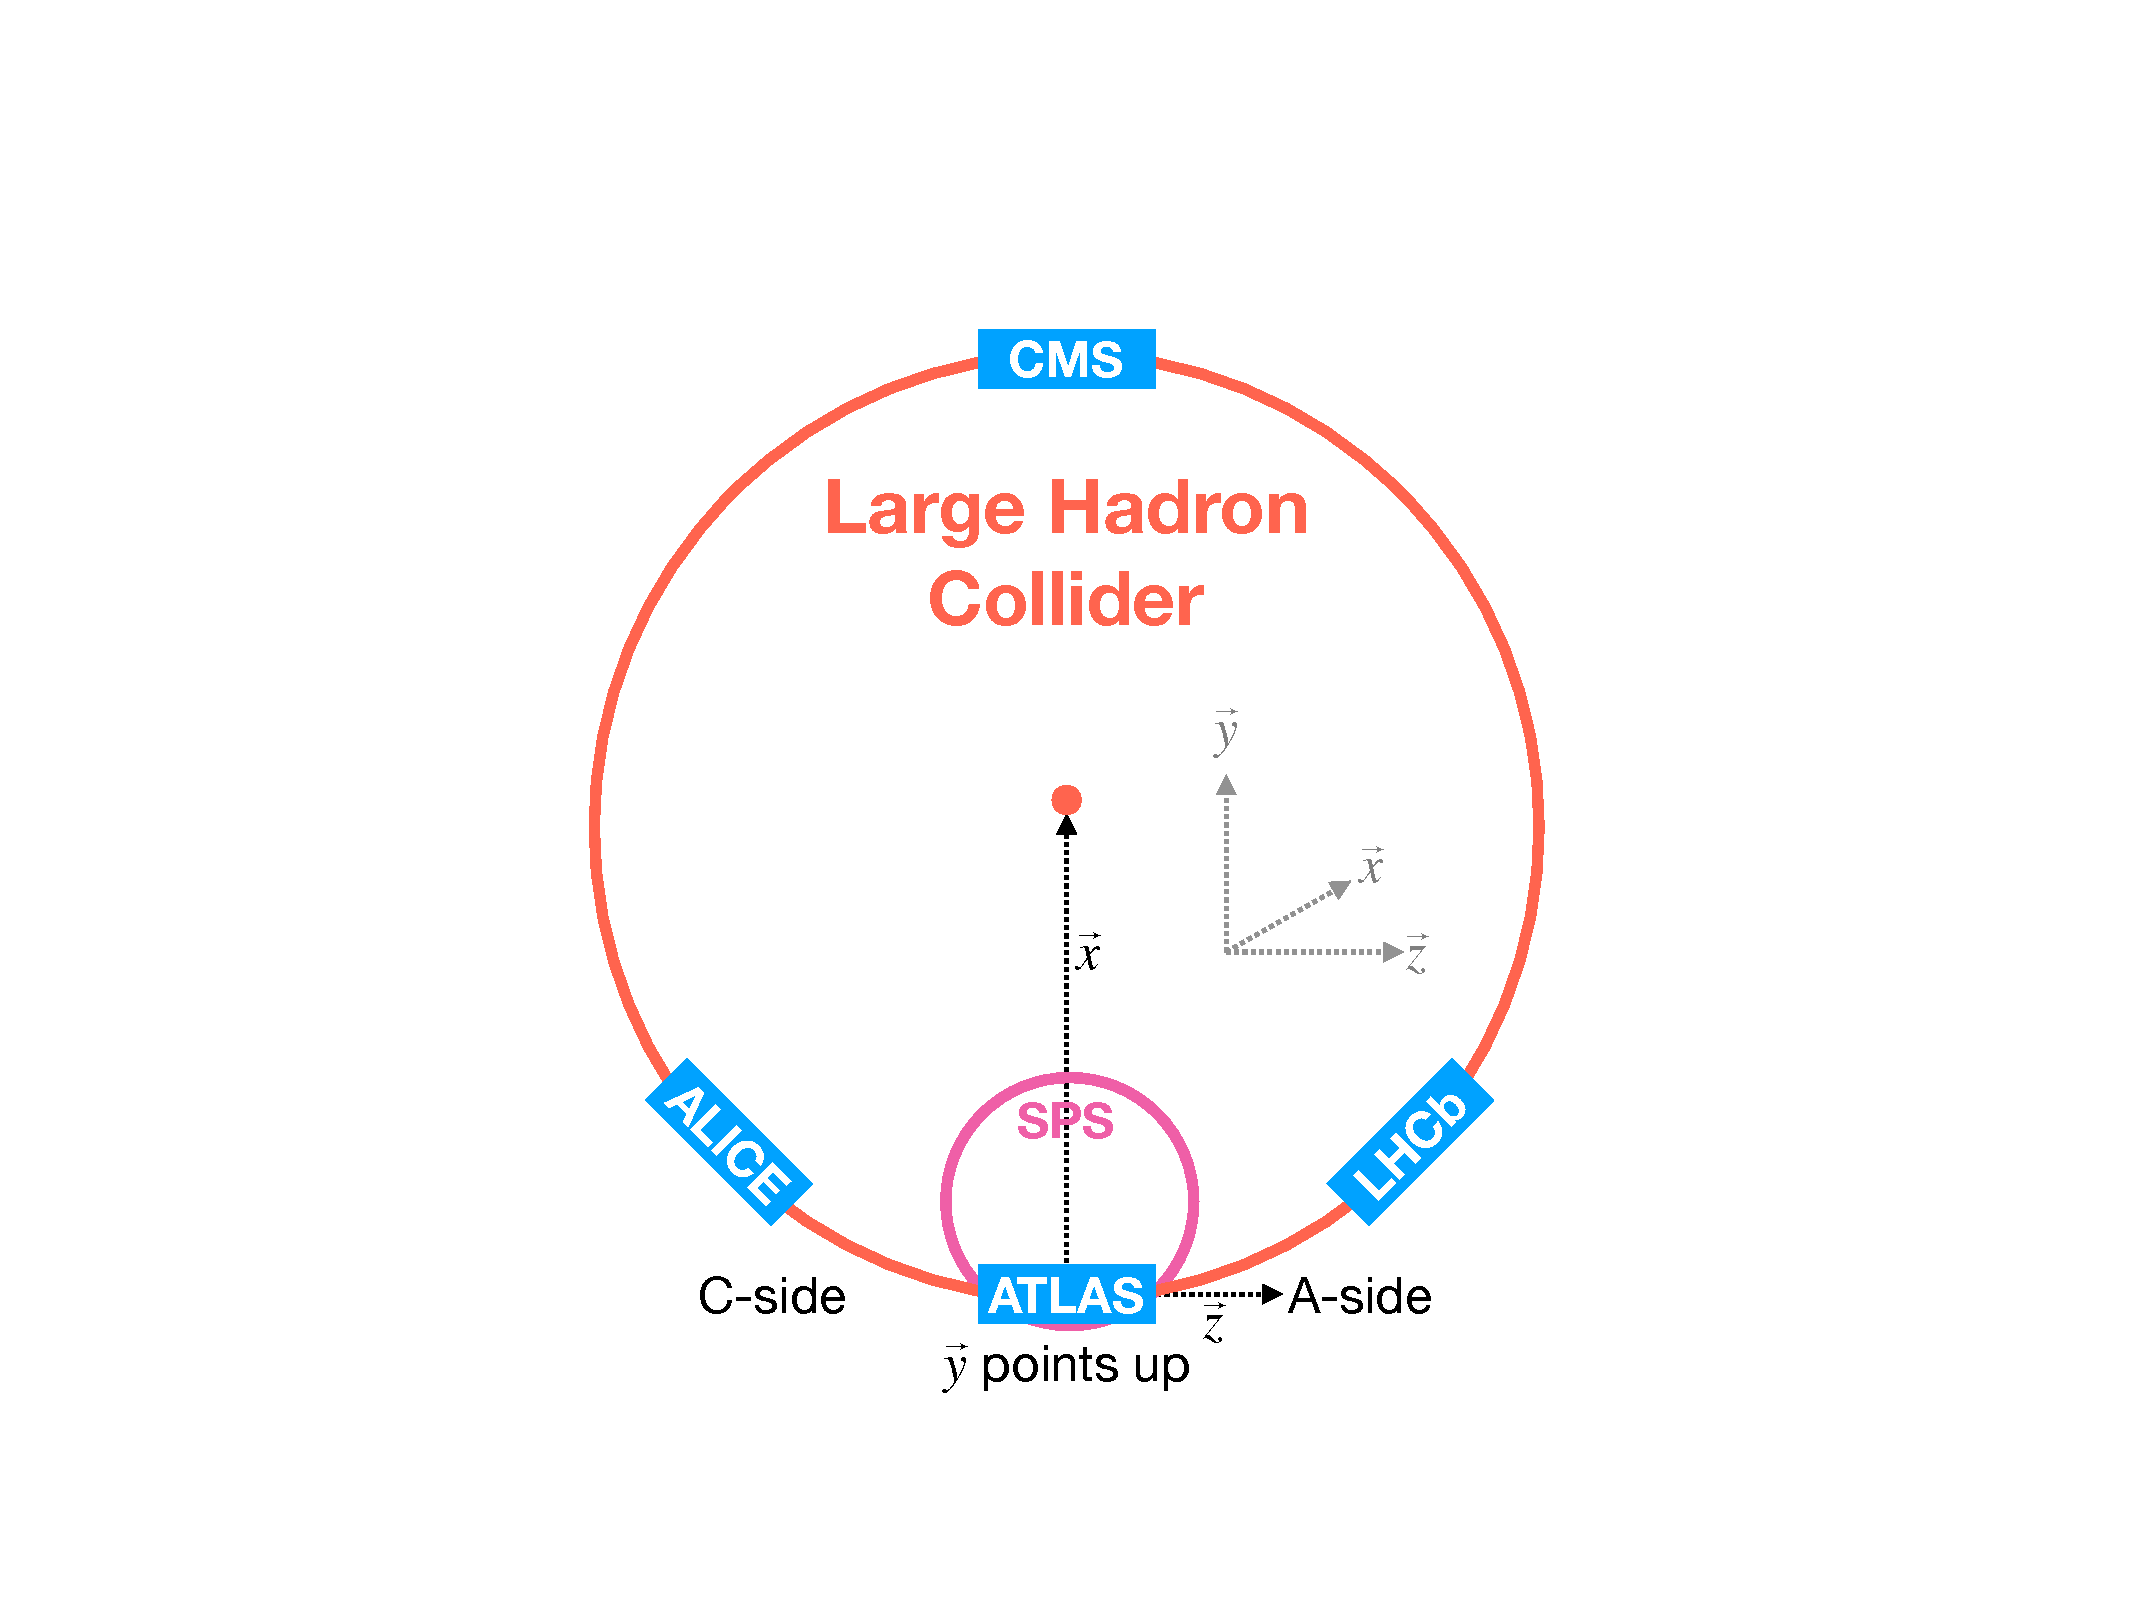
\includegraphics[width=0.5\linewidth]{figures/atlas/atlas_geometry}
    \caption{ \cite{Stark:2317296} A cartoon view of the the LHC from above
showing the SPS, LHC and the four main experiments of the LHC: ATLAS, CMS, LHCb,
and ALICE.  The standard cartesian coordinate system is shown with its origin at
the ATLAS interaction point, the positive $x$-axis towards the center of the
LHC, the positive $y$-axis pointing upwards, and the positive $z$-axis pointing
along the beamline towards the "A-side"}
    \label{fig:atlas_geometry}
  \end{center}
\end{figure}

Using these coordinates we can define the physical momentum of the objects
measured as $\vec{p} = (\pt,p_z)$ with \pt being the momentum of the object in
the transverse plane and $p_z$ the momentum along the beam axis. Given the
cylindrical symmetry of ATLAS it is desirable to define the polar angle
$\theta$ from the beam axis with the $r$-$\phi$ plane being perpendicular to that
axis. Since the particles we observe are relativistically boosted in the
$z$-axis it is desirable to use the Lorentz invariant quantity pseudorapidity
$(\eta)$ defined in terms of the polar angle by

\begin{equation}
 \eta = -\ln \tan \left( \frac{\theta}{2} \right).
\end{equation}

where $\eta = 0$ is in the $x$-$y$ plane and larger values of $|\eta|$ being
closer to the beam axis as can be seen in \cref{fig:pseudorapidity}.

\begin{figure}[!htbp]
  \begin{center}
    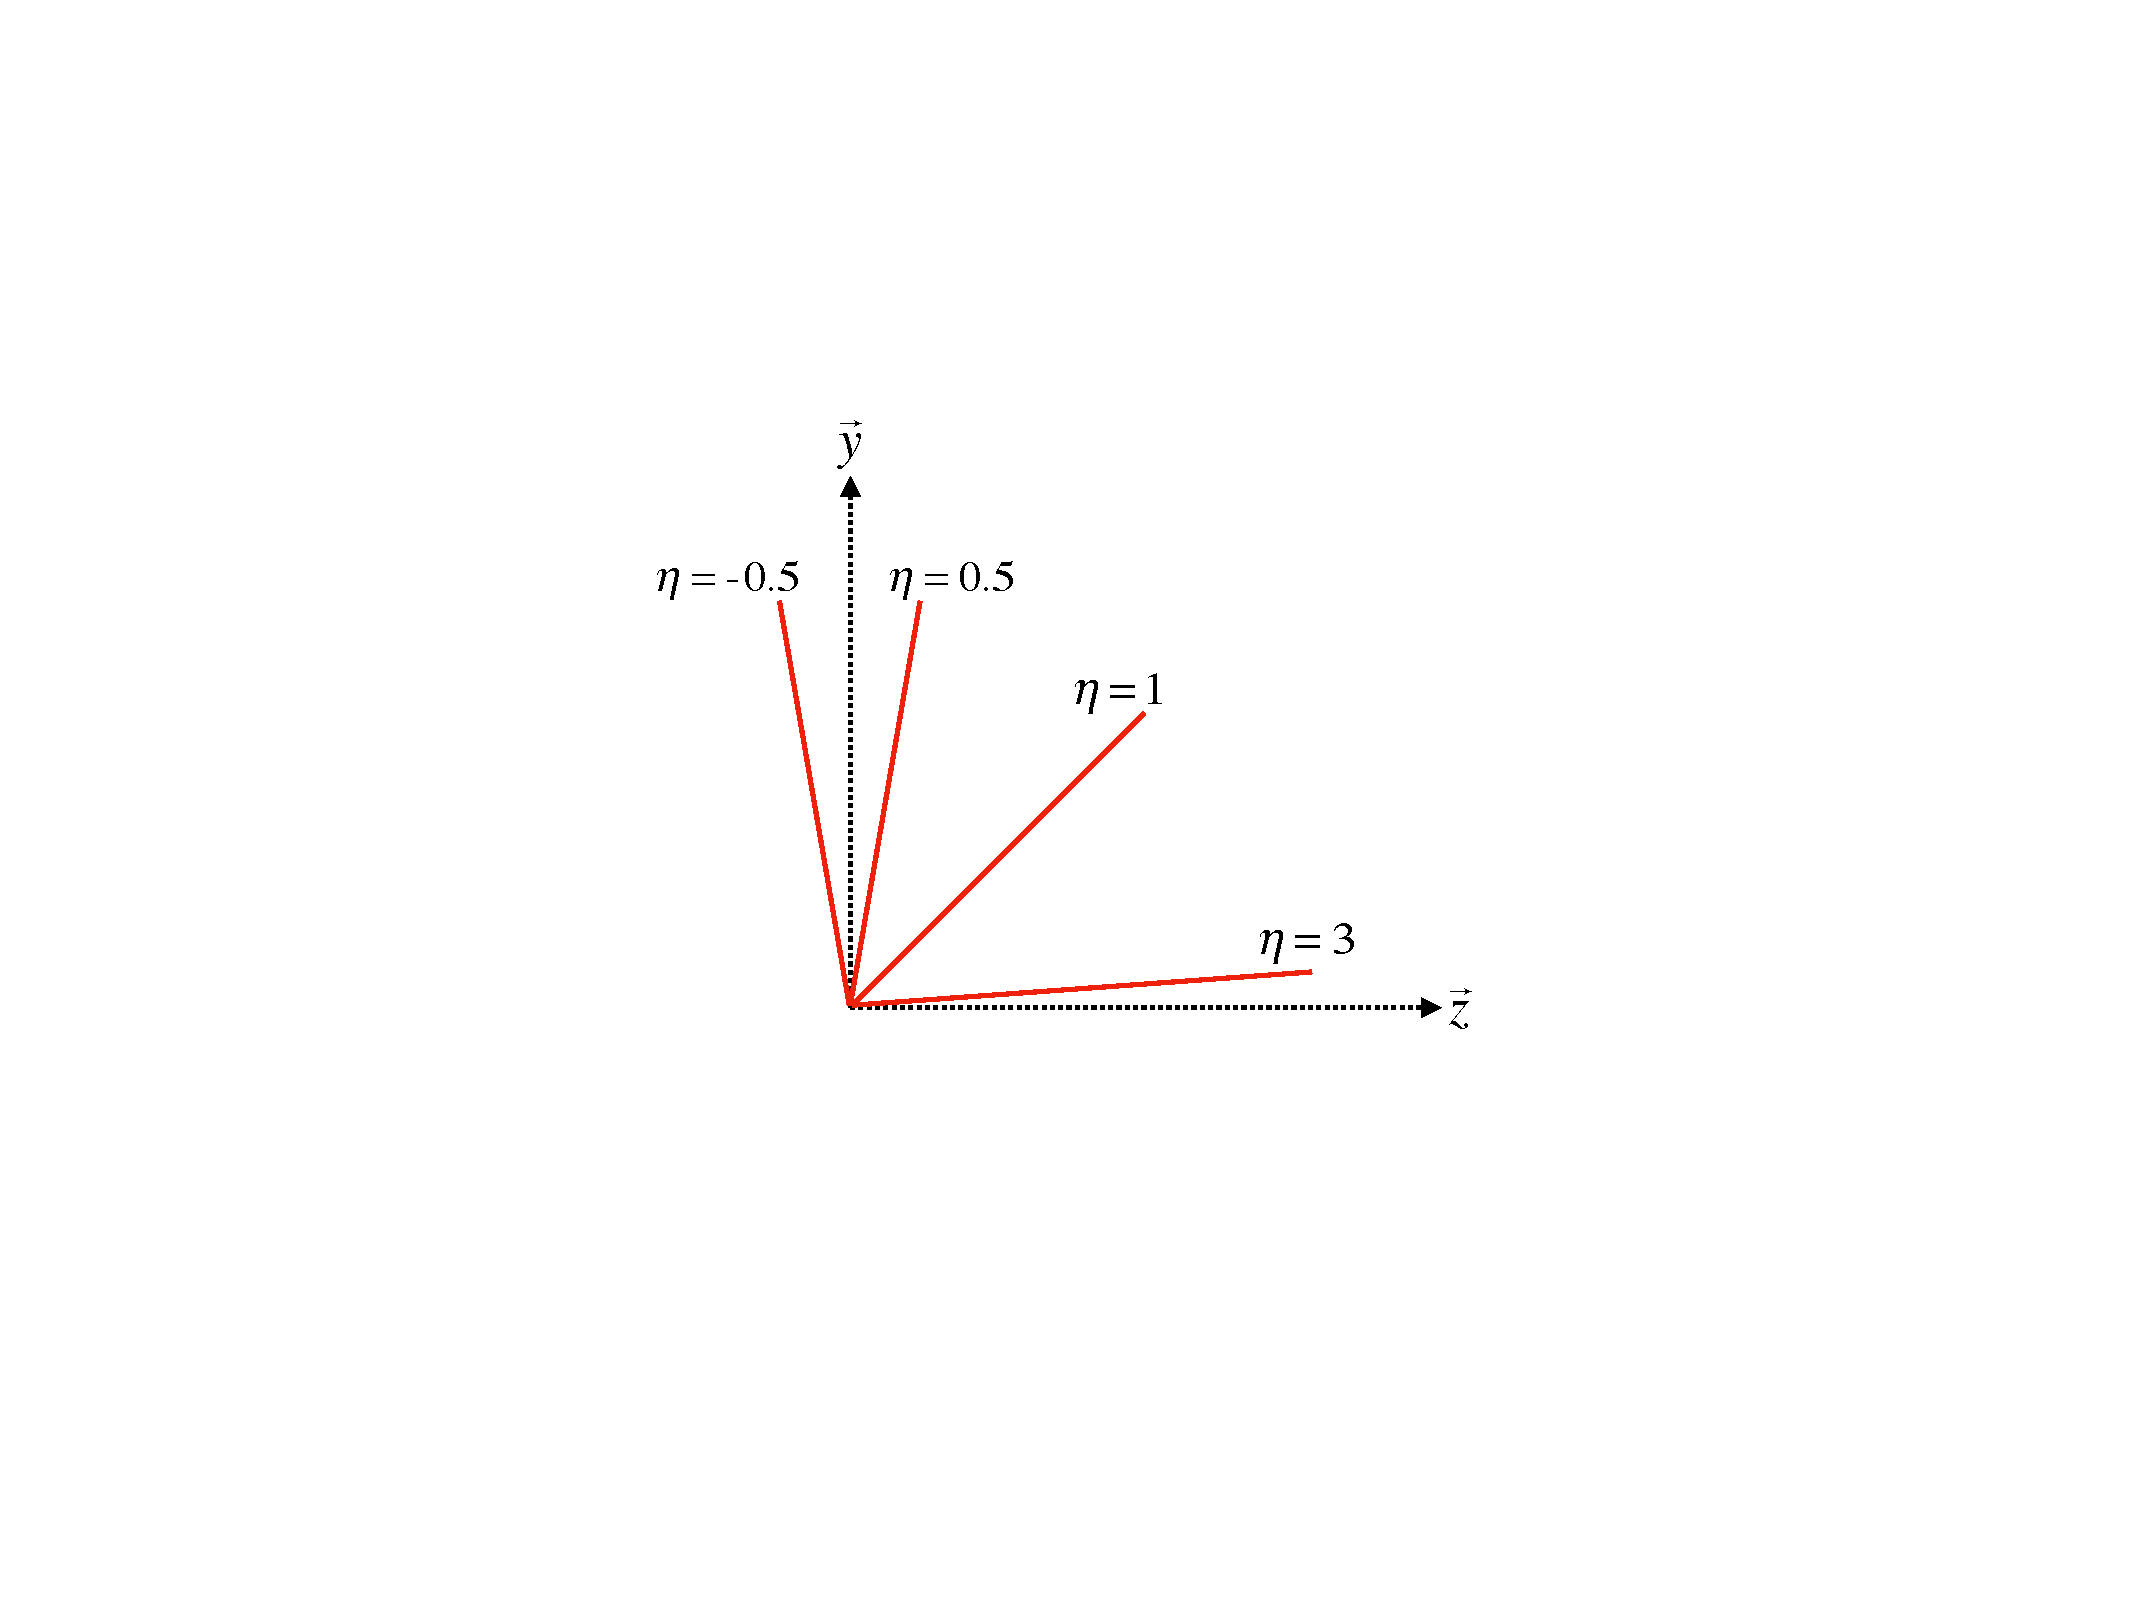
\includegraphics[width=0.5\linewidth]{figures/atlas/pseudorapidity}
    \caption{Modified from \cite{Stark:2317296} this cartoon represents a
selection of pseudorapiditity $(\eta)$ values overlaid with some cartesian
coordinates (dashed black lines).  The red lines are drawn for $\eta = \pm
0.5,1.0,3.0$ }
    \label{fig:pseudorapidity}
  \end{center}
\end{figure}

In this analysis the angular separation between objects in the detector is
calculated and represented using the geometric quantity 

\begin{equation}
 \DeltaRdef
\end{equation}
